\documentclass[letterpaper]{article}
\usepackage[square,sort,comma,numbers]{natbib}
\newcommand{\citeasnoun}[1]{Ref.~\citenum{#1}}

../../../../tex/scufftex.tex

\graphicspath{{figures/}}

%------------------------------------------------------------
%------------------------------------------------------------
%- Special commands for this document -----------------------
%------------------------------------------------------------
%------------------------------------------------------------
\newcommand{\vbhatt}[1]{\boldsymbol{\hat #1}}

%------------------------------------------------------------
%------------------------------------------------------------
%- Document header  -----------------------------------------
%------------------------------------------------------------
%------------------------------------------------------------
\title {Fields near RWG Panels}
\author {Homer Reid}
\date {August 27, 2014}

%------------------------------------------------------------
%------------------------------------------------------------
%- Start of actual document
%------------------------------------------------------------
%------------------------------------------------------------

\begin{document}
\pagestyle{myheadings}
\markright{Homer Reid: Fields near RWG panels}
\maketitle

In this note I discuss the evaluation of the
$\vb E$ and $\vb H$ fields due to RWG currents
on a single triangular source panel $\mc P$ in the case 
where the evaluation point lies on or near the source 
panel.
My method is essentially that of
Graglia\footnote{Graglia, \textit{IEEE Trans. Ant. Prop.} 
\textbf{41} 1448 (1993); see also 
Wilton et al., \textit{IEEE Trans. Ant. Prop.} \textbf{32} 
276 (1984).}; this is a desingularization scheme in which  
the first few terms in the low-frequency series expansion of the 
Green's function are subtracted off and evaluated analytically.
However, in {\sc scuff-em} I need also to compute the 
\textit{derivatives} of the $\vb E$ and $\vb H$ fields,
which requires an extension of Graglia's methods.

The algorithm described here is implemented in the 
file \texttt{GetNearFields.cc} in the {\sc scuff-em} source
distribution. 

\tableofcontents

%%%%%%%%%%%%%%%%%%%%%%%%%%%%%%%%%%%%%%%%%%%%%%%%%%%%%%%%%%%%%%%%%%%%%%
%%%%%%%%%%%%%%%%%%%%%%%%%%%%%%%%%%%%%%%%%%%%%%%%%%%%%%%%%%%%%%%%%%%%%%
%%%%%%%%%%%%%%%%%%%%%%%%%%%%%%%%%%%%%%%%%%%%%%%%%%%%%%%%%%%%%%%%%%%%%%
\newpage
\section{Fields from reduced potentials} 

%=================================================
%=================================================
%=================================================
\subsection{Reduced vector and scalar potentials}

Consider a triangular panel $\mc P$ on which we have a flow of 
surface current described by an RWG basis function
$\vb b_\alpha(\vb x)$ with source vertex $\vb Q$. I begin by
defining ``reduced'' vector and scalar potentials produced by this 
current at a point $\vb x$:
%====================================================================%
\numeq{ap}
{ \vb a(\mc P; \vb Q; \vb x) = \frac{\ell}{2A}
   \int_{\mc P} (\vb x^\prime - \vb Q) G(\vb x, \vb x^\prime) \, d\vb x^\prime,
   \qquad
   p(\mc P; \vb x) = 2\cdot\frac{\ell}{2A}
   \int_{\mc P} G(\vb x- \vb x^\prime) \, d\vb x^\prime,
}
%====================================================================%
where $\ell$ is the length of the edge associated with basis function
$\vb b$, $A$ is the area of $\mc P$, and
%====================================================================%
$$ G(\vb r)=\frac{e^{ik|\vb r|}}{4\pi |\vb r|} $$
%====================================================================%
is the scalar Helmholtz Green's function.

The total reduced vector and scalar potentials of $\vb b_\alpha$
involve contributions from two panels:
%====================================================================%
$$ \vb a_\alpha(\vb x) = \vb a(\mc P^+, \vb Q^+, \vb x) - 
                     \vb a(\mc P^-, \vb Q^-, \vb x), 
   \qquad 
   p_\alpha(\vb x) = p(\mc P^+, \vb Q^+, \vb x) - 
                     p(\mc P^-, \vb Q^-, \vb x).
$$
%====================================================================%
In terms of $\vb a_\alpha$ and $p_\alpha$, I can define the 
``reduced fields'' of basis function $\vb b_\alpha$ according to
%====================================================================%
\numeq{eh}
 { \vb e_\alpha(\vb x) 
   = \vb a_\alpha(\vb x) + \frac{1}{k^2} \nabla p_\alpha(\vb x), 
  \qquad 
  \vb h_\alpha(\vb x) = 
   \nabla \times \vb a_\alpha(\vb x)
 } 
%====================================================================%
Given a set of RWG functions $\{\vb b_\alpha\}$ populated
with electric and magnetic surface-current coefficients 
$\{k_\alpha, n_\alpha\}$, the full $\vb E$ and $\vb H$ fields at
$\vb x$ are 
%====================================================================%
\begin{align*}
 \vb E(\vb x) 
&= \sum_\alpha\Big\{  ikZ k_\alpha \vb e_\alpha(\vb x)
                     -n_\alpha \vb h_\alpha(\vb x)
              \Big\},
\\
 \vb H(\vb x) 
&= \sum_\alpha\Big\{  k_\alpha \vb h_\alpha(\vb x)
                     +\frac{ik}{Z} n_\alpha \vb e_\alpha(\vb x)
              \Big\}
\end{align*}
%====================================================================%
where $k$ is the wavenumber in the material region containing 
$\vb x$ and $Z=Z_0 Z^r$ with $Z_0$ the impedance of free space 
and $Z^r$ the relative wave impedance of the material.

To compute the first derivatives of the reduced fields we 
need the second derivatives of the reduced potentials:
%====================================================================%
$$ \partial_i e_j(\mc P^\pm; \vb x)
   =   \partial_i a_j(\mc P^\pm; \vb x) 
     + \frac{1}{k^2}\partial_i \partial_j p(\mc P^\pm, \vb c),
  \qquad
   \partial_i h_j(\mc P^\pm; \vb x)
   =\varepsilon_{jk\ell} \partial_i \partial_k a_\ell(\mc P^\pm; \vb x).
$$
%====================================================================%

%=================================================
%=================================================
%=================================================
\subsection{Desingularized reduced potentials}

To compute $\vb a$ and $p$ at evaluation points $\vb x$ 
on or near the source panel $\mc P$ it is convenient 
to invoke the expansion
%====================================================================%
\begin{align*}
 G(r) &= \frac{e^{ikr}}{4\pi r} 
       =  \frac{1}{4 \pi r} + (ik)\frac{1}{4 \pi}
         +(ik)^2 \frac{r}{8 \pi}
         +\frac{\texttt{ExpRelBar}(ikr,3)}{4\pi r}
\end{align*}
%====================================================================%
where \texttt{ExpRelBar} is just the usual exponential minus the 
first few terms in its series expansion:\footnote{\texttt{ExpRelBar}
is similar to, but distinct from, the function named \texttt{ExpRel} 
in the {\sc gnu scientific library.}}
%====================================================================%
$$ \texttt{ExpRelBar}(x,N) = e^{x}-\sum_{n=0}^{N-1}\frac{x^n}{n!}
                           = \sum_{n=N}^{\infty}\frac{x^n}{n!}.
$$
%====================================================================%
The reduced potentials due to $\mc P$ are
%====================================================================%
\begin{align*}
 p(\vb x) 
   &= 2\frac{\ell}{2A} \left[
\sum_{n=-1}^1 \frac{(ik)^{n+1}}{4\pi} p^{(n)}(\vb x)
      + p\supt{DS}(\vb x)
                       \right]
\\
 \vb a(\vb x) 
   &=  \frac{\ell}{2A} \left[
      \sum_{n=-1}^1 \frac{(ik)^{n+1}}{4\pi} \vb a^{(n)}(\vb x)
      + \vb a \supt{DS}(\vb x)
                       \right]
\end{align*}
%====================================================================%
where\footnote{Two special cases that may be computed
analytically are $p^{(0)}=A, \vb a^{(0)}=A(\vb x_c - \vb Q)$
where $A$ is the panel area and $\vb x_c$ is its centroid. These
are independent of the evaluation point $\vb x$ and thus do not 
contribute to derivatives.}
%====================================================================%
\begin{align}
 p^{(n)}(\vb x) &= \int_{\mc P} r^n \, dA
\label{pnDef} \\
%--------------------------------------------------------------------%
 \vb a^{(n)}(\vb x)
&= \int_{\mc P} (\vb x^\prime - \vb Q)r^n \, dA.
\label{anDef}
%%--------------------------------------------------------------------%
\intertext{(here $r=|\vb x^\prime - \vb x|$).
           To write $\vb a^{(n)}$ in a more convenient form, let
           $\overline{\vb x}$ be the projection of the evaluation point
           into the plane of the panel and write}
%--------------------------------------------------------------------%
\vb a^{(n)}(\vb x)
&= \int_{\mc P}
   \Big( \vb x^\prime - \overline{\vb x} + \overline{\vb x} - \vb Q \Big)
   r^n \, dA
\nn
%--------------------------------------------------------------------%
&= \int_{\mc P} 
   \Big( \vb x^\prime - \overline{\vb x} \Big) r^n \, dA
   -(\vb Q - \overline{\vb x}) \int_{\mc P} r^n dA.
\nonumber
\end{align}
%====================================================================%
To proceed I now define scalar and vector-valued functions according 
to\footnote{Note that I use a $p$ superscript for $\mc I$ and $\bmc J$
but an $(n)$ superscript for $\vb a$ and $p$. This is because the 
indices $p$ and $n$ have different ranges: The $n$ values for which I 
need $\vb a^{(n)}$ and $p^{(n)}$ and their derivatives are 
$n={-1,0,1}$, but computing all of these quantities turns out to 
require $\mc I^p$ and $\bmc J^p$ for $p={-5,-3,-1,1}.$}
%====================================================================%
\begin{subequations}
\begin{align}
 I^p(\mc P, \vb x) &\equiv 
 \int_{\mc P} r^p \, dA
\\
\bmc J^p(\mc P, \vb x)
 &\equiv \int_{\mc P} \overline{\vb r} \cdot  r^p \, dA.
\label{IJIntegralDefinition}
\end{align}
\end{subequations}
%====================================================================%
where $\overline{\vb r}=\vb x^\prime-\overline{\vb x}$ 
is a vector that has nonzero components only in the plane of $\mc P$.
%====================================================================%
In terms of $\mc I$ and $\mc J$, the reduced potentials are
%====================================================================%
\numeq{paFromIJ}
{
  p^{(n)}(\mc P; \vb x) = \mc I^n(\mc P; \vb x),
   \qquad
   \vb a^{(n)}(\mc P; \vb x) =
   \bmc J^n(\mc P; \vb x)
      - \big(\vb Q-\overline{\vb x}\big) \mc I^n(\mc P; \vb x)
}
%====================================================================%
Similarly, derivatives of $\vb a^{(n)}$ and $p^{(n)}$ are related to 
derivatives of $\mc I^p$ and $\bmc J^p$:
%====================================================================%
\begin{align*}
 \partial_i p^p (\vb x) &= d_i \mc I^p(\mc P, \vb x) 
\\
 \partial_i a^p_j (\vb x)
&= \partial_i \mc J_j^p(\mc P, \vb x)
  -(\vb Q - \overline{\vb x})_j \partial_i \mc I^p
  -\delta_{ij} \mc I^p(\mc P, \vb x)
\end{align*}
%====================================================================%

The two-dimensional integrals in the quantities $\mc I^p$
and $\bmc J^p$ defined by Equation (\ref{IJIntegralDefinition}),
as well as their derivatives, may be evaluated analytically in 
closed form, as discussed in the following section.

%%%%%%%%%%%%%%%%%%%%%%%%%%%%%%%%%%%%%%%%%%%%%%%%%%%%%%%%%%%%%%%%%%%%%%
%%%%%%%%%%%%%%%%%%%%%%%%%%%%%%%%%%%%%%%%%%%%%%%%%%%%%%%%%%%%%%%%%%%%%%
%%%%%%%%%%%%%%%%%%%%%%%%%%%%%%%%%%%%%%%%%%%%%%%%%%%%%%%%%%%%%%%%%%%%%%
\newpage
\section{Evaluation of $\mc I, \bmc J$ integrals}

%=================================================
%=================================================
%=================================================
\subsection{Modified coordinate system}
%####################################################################%
\begin{figure}
\begin{center}
\resizebox{\textwidth}{!}{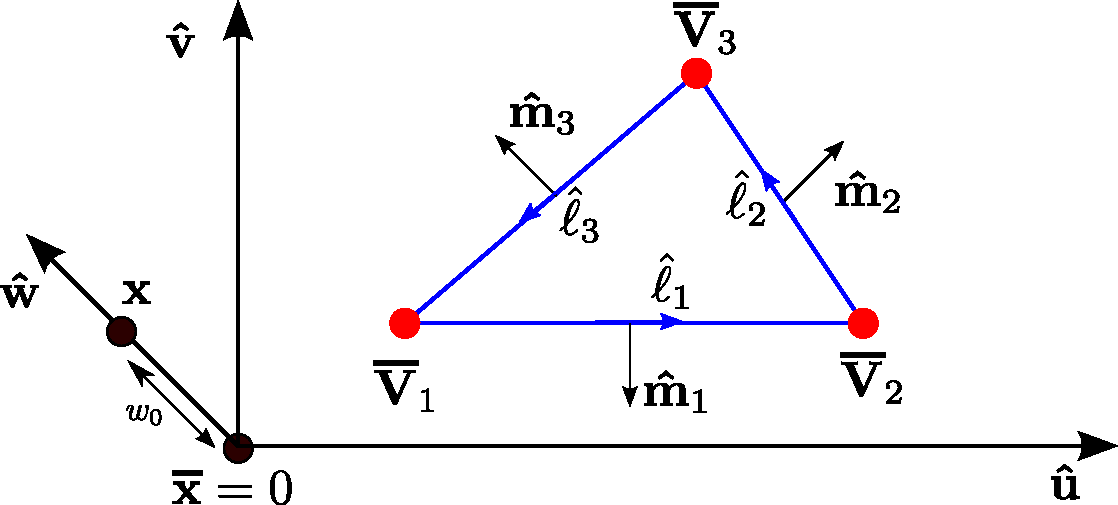
\includegraphics{NearFieldUVWSystem.pdf}}
\caption{Rotated and translated coordinate system 
         ($\vbhat{u},\vbhat{v},\vbhat{w}$) for evaluation of 
         $\mc I, \bmc J$ integrals. The panel lies in the $uv$ plane
         with one edge parallel to the $\vbhat{u}$ axis. The origin
         of the $uv$ plane is the projection of the evaluation point
         into the plane of the panel. The perpendicular distance from
         the plane of the panel to the evaluation point is $w_0$.}
\label{UVWSystemFigure}
\end{center}
\end{figure}
%####################################################################%

Let the panel $\mc P$ have vertices
$\{\vb V_1, \vb V_2, \vb V_3\}.$
For convenience in what follows, we introduce a
rotated and translated coordinate system with 
cartesian coordinates
$(u,v,w)$, in which $\mc P$ lies entirely in the $uv$
plane (the panel normal $\vbhat{n}$ defines the $\vbhat{w}$ axis)
and edge $\vb V_1 \vb V_2$ lies parallel to the 
$\vbhat{u}$ axis (Figure \ref{UVWSystemFigure}).
The unit vectors of this system 
are 
%====================================================================%
$$ \vbhat{u}=\frac{\vb V_2 - \vb V_1}{|\vb V_2 - \vb V_1|},
   \qquad
   \vbhat{v}=\vbhat{w} \times \vbhat{u},
   \qquad
   \vbhat{w}=
    \frac{ (\vb V_2 - \vb V_1)\times(\vb V_3 - \vb V_1)}
         {|(\vb V_2 - \vb V_1)\times(\vb V_3 - \vb V_1)|}
$$
%====================================================================%
In the modified coordinate system, the evaluation point has
coordinates $\vb x = (\vbrho_0, w_0)$ with
%====================================================================%
$$ w_0 = (\vb x_0 - \vb x_c) \cdot \vbhat{w}, 
   \qquad
   \vbrho_0 = (\vb x_0 - \vb x_c) - w_0\vbhat{w}
$$
%====================================================================%
(where $\vb x_c$ is the centroid of $\mc P$).
It is convenient to choose the origin of the $(u,v)$ plane to be 
the point $\vbrho_0$. The $(u,v,w)$ coordinates of the $i$th 
panel vertex are then 
$\overline{\vb V}_i = (u_i, v_i, 0)$ where
%====================================================================%
$$ u_i=(\vb V_i-\vb x_c) \cdot \vbhat{u}, \qquad 
   v_i=(\vb V_i-\vb x_c) \cdot \vbhat{v}.
$$
%====================================================================%
I also define a two-dimensional 
unit vector $\vbhatt{\ell}_i$ pointing in the direction
of the $i$th panel edge according to
%====================================================================%
$$ \vbhatt{\ell}_i= \frac{  \overline{\vb V}_{i+1}-\overline{\vb V}_{i} }
                         { |\overline{\vb V}_{i+1}-\overline{\vb V}_{i}| }
$$
%====================================================================%
and a two-dimensional unit vector $\vbhat{m}_i$ normal to the $i$th 
panel edge according to 
%====================================================================%
$$ \vbhat{m}_i=\vbhat{w} \times \vbhatt{\ell}_i.$$
%====================================================================%

%=================================================
%=================================================
%=================================================
\subsection{Reduction of surface integrals to line integrals}

I now convert the two-dimensional (surface) integrals 
$\{\mc{I}, \bmc J\}^p$ defined by (\ref{IJIntegralDefinition})
into one-dimensional (line) integrals by using Stokes' theorem in the forms
%====================================================================%
\begin{subequations}
\begin{align}
 \int_{\mc P} \nabla \cdot \vb f(\vbrho)\,dA
 &=
 \oint_{\partial \mc P} \vb f(\vbrho) \cdot \vbhat{m} \, d\ell
\\
 \int_{\mc P} \nabla f(\vbrho)\,dA
 &=
 \oint_{\partial \mc P} f(\vbrho) \, \vbhat{m} \, d\ell.
\end{align}
\label{Stokes}
\end{subequations}
%====================================================================%
[Here $\vbrho=(u,v)$.]

First consider the vector-valued function
$$ \vb f(\vbrho)=
   \frac{1}{p+2}
   \frac{ [\rho^2 + w^2]^{(p+2)/2}}{\rho}\vbhatt{\rho} $$
with divergence
%====================================================================%
$$
   \nabla \cdot \vb f(\vbrho)=
   \frac{1}{\rho}\pard{}{\rho}\Big(\rho f_\rho(\vbrho) \Big)
   = [\rho^2 + w^2]^{p/2}.
$$
%====================================================================%
Applying (\ref{Stokes}a) to this function yields
%====================================================================%
$$\mathcal{I}^p
  \equiv \int_{\mc P} [\rho^2 + w^2]^{p/2} dA
  =\frac{1}{(p+2)}\int_{\partial \mc P} 
   \frac{ [\rho^2 + w^2]^{(p+2)/2} } { \rho } 
   \vbhatt{\rho}\cdot\vbhat{m} \, d\ell.
$$
%====================================================================%
Next consider the scalar function 
%====================================================================%
$$ f(\rho) = \frac{1}{p+2} [\rho^2 + w^2]^{ (p+2)/2} $$
%====================================================================%
with gradient
%====================================================================%
$$ \nabla f(\rho) = \vbrho [\rho^2 + w^2]^{p/2}.$$
%====================================================================%
Applying (\ref{Stokes}b) to this function yields
%====================================================================%
$$\bmc{J}^p
  \equiv  \int_{\mc P} \vbrho \cdot r^p dA
  =\frac{1}{(p+2)}\int_{\partial \mc P}
   [\rho^2 + w^2]^{(p+2)/2}  \vbhat{m} \, d\ell.
$$
%====================================================================%

%=================================================
%=================================================
%=================================================
\subsection{Evaluation of line integrals} 

Line integrals are sums of integrals over line segments (edges).
On edge $i$, we have 
$$ \vbrho(s,t_i)=s\vbhatt{\ell}_i - t_i\vbhat{m}_i, 
   \qquad 
   \rho(s,t_i) = \sqrt{s^2 + t_i^2},
   \qquad 
   \vbhatt{\rho}\cdot \vbhat{m} = -\frac{t_i}{\rho}.
$$
Here $t_i$ is the perpendicular distance from edge 
$\overline{\vb V}_{i}\overline{\vb V}_{i+1}$ to the origin
and $s$ runs from $s_i^-$ to $s_i^+$, where
%====================================================================%
\begin{align*}
 t_i   &= -\vb V_i \cdot \vbhat{m}_i = -\vb V_{i+1}\cdot \vbhat{m}_i
\\
 s_i^- &= \vb V_i \cdot \vbhatt{\ell}_i
\\
 s_i^+ &= \vb V_{i+1} \cdot \vbhatt{\ell}_i
\end{align*}
%====================================================================%
Then we have
\begin{align*}
 \mathcal{I}^p
&=\frac{1}{(p+2)} \int_{\partial \mc P} 
   \frac{ [\rho^2 + w^2]^{(p+2)/2} } { \rho }
   \vbhatt{\rho}\cdot \vbhat{m}\,d\ell
\\
&=-\frac{1}{(p+2)}
   \sum_i \underbrace{t_i\int_{s_i^-}^{s_i^+} 
                \frac{ (s^2 + t_i^2 + w^2)^{(p+2)/2}}{(s^2 + t_i^2)}ds}
               _{I^p(s_i^-, s_i^+, t_i, w)}
\\
 \bmc {J}^p
&= \frac{1}{(p+2)}
   \int_{\partial \mc P} [\rho^2 + w^2]^{(p+2)/2}
   \vbhat{m} \, d\vbhatt{\ell}
\\
&= \frac{1}{(p+2)} \sum_i \vbhat{m}_i 
    \underbrace{ \int_{s_i^-}^{s_i^+} [s^2 + t_i^2 + w^2]^{(p+2)/2}ds}
                 _{J^p(s_i^-, s_i^+, t_i,w)}.
\end{align*}
%====================================================================%
The one-dimensional integrals defining $I^p$ and $J^p$ may be evaluated
in closed form:
%====================================================================%
$$\begin{array}{|c|c|c|}\hline
%--------------------------------------------------------------------%
p 
& 
I^p(s^-, s^+, t, w)
&
J^p(s^-, s^+, t, w)
\\\hline
%--------------------------------------------------------------------%
-5 
&
\frac{t}{w^2 X^2}\left( \frac{s^-}{R^-} - \frac{s^+}{R^+} \right)
+\frac{\zeta}{w^3} 
&
\frac{1}{X^2}\left( \frac{s^+}{R^+} - \frac{s^-}{R^-} \right)
\\\hline
%--------------------------------------------------------------------%
-3 
&
\frac{\zeta}{w}
&
\Lambda
\\\hline
%--------------------------------------------------------------------%
-1 
&
w\zeta + t\Lambda
&
\frac{1}{2}\Big(R^+ s^+ - R^- s^- + X^2 \Lambda\Big)
\\\hline
%--------------------------------------------------------------------%
+1 
&
\frac{t}{2}\Big[R^+ s^+ - R^- s^- + \Lambda(t^2 + 3w^2)\Big]
 + w^3 \zeta
&
\parbox{0.4\textwidth}{$
\frac{1}{8}\Big[2R^+ s^{+3} - 2R^- s^{-3} + 5X^2(R^+ s^+ - R^- s^-)
 + 3\Lambda X^4\Big]$}
\\\hline
\end{array}$$
%====================================================================%

In this table, we have used the following shorthand:
%====================================================================%
\begin{align*}
 X&=\sqrt{t^2 + w^2},
 \qquad
 R^+=\sqrt{s^{+2} + X^2},
 \qquad
 R^-=\sqrt{s^{-2} + X^2}
\\
 Z^+ &= R^+ + s^+ 
\qquad 
 Z^- = R^- + s^-
\\
 \Lambda &= \log\frac{Z^+}{Z^-}, \qquad 
 \zeta   = \atan\pf{w s^+}{tR^+} - \atan\pf{w s^-}{tR^-}
\end{align*}
%====================================================================%

%=================================================
%=================================================
%=================================================
\subsection{Derivatives of reduced potentials}

\subsubsection{Potential derivatives from $\mc I,J$ derivatives}

When computing derivatives it is easiest to work first
in the $\vbhat{u},\vbhat{v},\vbhat{w}$ coordinate system 
and later rotate back to the original coordinate system.
In this case, in-plane derivatives (derivatives with respect
to the $u,v$ coordinates) are distinguished from 
normal derivatives (derivatives with respect to the $w$ 
coordinate).
To highlight this distinction, in what follows the subscripts 
$\alpha,\beta,\gamma$ will refer only to the in-plane coordinates
($u,v$ coordinates), so that e.g. $\partial_\alpha \mc I$ refers 
to an in-plane derivative, while $\partial_w \mc I$ is a 
normal derivative. Note that the vector potential $\vb a$, 
like the quantities $\bmc J$ and $\vb Q$, has only
in-plane components.

The starting point is equation (\ref{paFromIJ}):
$$ p^{(n)} = \mc I^n, 
   \qquad 
   a_\gamma^{(n)} = \mc J^n_\gamma - \overline{\vb Q}_\gamma \mc I^n
$$
Derivatives of $p$ are just derivatives of $\mc I$,
computed as discussed below.

First derivatives of $\vb a$ take the form
%====================================================================%
\begin{align*}
 \partial_\beta a_\gamma^{(n)}
&=   \partial_\beta \mc J^n_\gamma
   + n\overline{\vb Q}_\gamma \mc J^{n-2}_\beta
   + \delta_{\beta\gamma} \mc I^n
\\
 \partial_w a_\gamma^{(n)}
&=   \partial_w \mc J^n_\gamma
   - \overline{\vb Q}_\gamma \partial_w \mc I^n
\\
&=   nw\big[    \mc J^{n-2}_\gamma
              - \overline{\vb Q}_\gamma \mc I^{n-2}
       \big]
\end{align*}
%====================================================================%
When computing second derivatives of $\vb a$, it turns
out that the double normal derivative $\partial^2_w a_\gamma$
and the mixed second partial $\partial_w \partial_\alpha \vb a_\gamma$
are straightforward to compute in terms of $\mc I,\bmc J$
and their first derivatives:
%====================================================================%
\begin{align*}
 \partial_w \partial_\beta a_\gamma^{(n)}
&= (n-2)w \Big[ \partial_\beta \bmc J_\gamma^{(n-2)}
               +n\overline{\vb Q}_\gamma \mc J_\beta^{n-4}
          \Big]
   +nw \delta_{\beta\gamma} \mc I^{n-2}
\\
 \partial_w^2 a_\gamma^{(n)}
&=   n\big[    \mc J^{n-2}_\gamma
             - \overline{\vb Q}_\gamma \mc I^{n-2}
      \big]
\\
&\qquad
  +n(n-2) w^2 
   \Big[ \mc J^{n-4}_\gamma -\overline{\vb Q}_\gamma \mc I^{n-4}\Big]
\end{align*}
%====================================================================%
The double in-plane derivative $\partial_\alpha \partial_\beta a_\gamma$ 
is more difficult to compute. However,
it turns out we don't need to compute this quantity as long as 
we are only interested in first derivatives of the 
$\vb E$ and $\vb H$ fields. To see this, note that second 
derivatives of $\vb a$ only enter in the computation of 
first derivatives of $\vb H$, which involves differentiating
the curl of $\vb a$. In the $(uvw)$ system, the curl of $\vb a$ 
reads
%====================================================================%
\begin{align*}
 \nabla\times \vb a
 &= -\partial_w a_v \vbhat{u} 
    +\partial_w a_u \vbhat{v} 
    +(\partial_u a_v - \partial_v a_u) \vbhat{w}
\end{align*}
%====================================================================%
The $w$ derivative of this is 
%====================================================================%
\begin{align*}
 \partial_w (\nabla \times \vb a)
  &= -\partial^2_w a_v \vbhat{u} 
     +\partial^2_w a_u \vbhat{v} 
    +(\partial_w \partial_u a_v - \partial_w \partial_v a_u) \vbhat{w}
\end{align*}
which does not require the double in-plane derivative.
%====================================================================%
The in-plane derivative of $\nabla \times a$ is
%====================================================================%
\begin{align*}
 \partial_\alpha (\nabla \times \vb a)
  &= -\partial_\alpha \partial_w a_v \vbhat{u}
     +\partial_\alpha \partial_w a_u \vbhat{v} 
    +(\partial_\alpha \partial_u a_v - \partial_\alpha \partial_v a_u) 
     \vbhat{w}
\end{align*}
%====================================================================%
To elucidate the structure of the $w$ component of this, I write
%====================================================================%
\newcommand{\xbar}{\big(\overline{\vb x}\big)}
\newcommand{\Qbar}{\big(\overline{\vb Q}\big)}
\newcommand{\xmQ}{\big(\overline{\vb x} - \overline{\vb Q}\big)}
\begin{align*}
 \partial_u a_v^{(n)} - \partial_v a_u^{(n)}
&= -n\int
    \underbrace{\Big[\xbar_u \xmQ_v - \xbar_v \xmQ_u\Big]} 
              _{\Qbar_u \xbar_v - \Qbar_v \xbar_u} r^{n-2}  \, dA
\\
&= -n\Big[ \Qbar_u \int \xbar_v r^{n-2} \, dA
          -\Qbar_v \int \xbar_u r^{n-2} \, dA
     \Big]\\
&= -n\Big[\Qbar_u \mc J_v^{n-2} - \Qbar_v \mc J_u^{n-2}\Big]
\intertext{and thus}
 \partial_\alpha(\nabla \times \vb a)_w
&= -n\Big[    \Qbar_u \partial_\alpha \mc J_v^{n-2} 
            - \Qbar_v \partial_\alpha \mc J_u^{n-2}
     \Big].
\end{align*}
The upshot is that all quantities needed to compute
first and second derivatives of the potentials may be 
obtained from the $\mc I, J$ integrals and their 
first derivatives.

\subsubsection{Derivatives of $\mc I,J$ integrals}

(In what follows, subscripts $\mu,\nu$ refer to derivatives
with respect to coordinates in the plane of the panel [$u,v$
derivatives in the $(u,v,w)$ system], as distinct from 
$w$ derivatives, which are directional derivatives in the 
direction normal to the panel.)

Derivatives of the $\mc I$ integrals, and the normal derivative
of the $\mc J$ integrals, may be carried out at the level of surface
integrals:

%====================================================================%
\begin{align*}
%--------------------------------------------------------------------%
 \partial_\mu \mc I^p(\vb x)
&= \partial_\mu \int_{\mc P} [\rho^2 + w^2]^{p/2}\,dA
 =-p \int_{\mc P} 
   \rho_\mu [\rho^2 + w^2]^{(p-2)/2}\,dA
\\
%--------------------------------------------------------------------%
&=-p\mc J_\mu^{p-2}(\vb x)
\\[8pt]
%--------------------------------------------------------------------%
 \partial_w \mc I^p(\vb x)
&= \partial_w \int_{\mc P} [\rho^2 + w^2]^{p/2}\,dA
 =pw \partial_w \int_{\mc P} [\rho^2 + w^2]^{(p-2)/2}\,dA
\\
%--------------------------------------------------------------------%
&=pw\mc I^{p-2}(\vb x)
\intertext{and similarly}
 \partial_w \bmc J^p(\vb x)
&=pw \bmc J^{p-2}(\vb x)
\end{align*}
%====================================================================%

In-plane derivatives of the $\mc J$ integrals are easiest to carry out at
the level of line integrals:
%====================================================================%
\begin{align*}
 \partial_\mu \mc J_\nu^p(\vb x)
&=\frac{1}{(p+2)} \sum_i 
  \left\{  \Big( \partial_\mu J^p \Big) \hat{m}_{i\nu}
  \right\}
\\
%--------------------------------------------------------------------%
  \partial_\mu J^p(s_i^-, s_i^+, t_i, w)
&= \left[
   \pard{J^p}{\vbhatt{\ell}_i} \vbhatt{\ell}_i
  +\pard{J^p}{\vbhat{m}_i} \vbhat{m}_i
   \right]
\\
   \pard{J^p}{\vbhatt{\ell}_i}
&= -(s_i^{-2} + t_i^2 + w^2)^{(p+2)/2}
   -(s_i^{+2} + t_i^2 + w^2)^{(p+2)/2}
\\
   \pard{J^p}{\vbhatt{m}_i}
&= (p+2) t_i J^{p-2}
\\
\end{align*}
%====================================================================%

\subsubsection{Derivatives of desingularized terms}

We have
%====================================================================%
\begin{align*}
 G\supt{DS}(r) &= \frac{\texttt{ExpRelBar}(ikr,3)}{4\pi r}
\\
\intertext{and thus}
\partial_i 
 G\supt{DS}(r) &= 
       r_i  \Big[ ik\frac{\texttt{ExpRelBar}(ikr,2)}{4\pi r^2}
                   -\frac{\texttt{ExpRelBar}(ikr,3)}{4\pi r^3}
            \Big]
\\
\partial_i \partial_j
 G\supt{DS}(r) &= 
  \delta_{ij} \Big[ ik \frac{\texttt{ExpRelBar}(ikr,2)}{4\pi r^2}
                   -\frac{\texttt{ExpRelBar}(ikr,3)}{4\pi r^3}
              \Big]
\\
&\qquad 
 +r_i r_j   \Big[ (ik)^2 \frac{\texttt{ExpRelBar}(ikr,1)}{4\pi r^3}
                  -3ik\frac{\texttt{ExpRelBar}(ikr,2)}{4\pi r^4}
                  +3\frac{\texttt{ExpRelBar}(ikr,3)}{4\pi r^5}
            \Big]
\end{align*}
%====================================================================%

%%%%%%%%%%%%%%%%%%%%%%%%%%%%%%%%%%%%%%%%%%%%%%%%%%%%%%%%%%%%%%%%%%%%%%
%%%%%%%%%%%%%%%%%%%%%%%%%%%%%%%%%%%%%%%%%%%%%%%%%%%%%%%%%%%%%%%%%%%%%%
%%%%%%%%%%%%%%%%%%%%%%%%%%%%%%%%%%%%%%%%%%%%%%%%%%%%%%%%%%%%%%%%%%%%%%
\newpage
\section{Far fields at nearby points}

The contribution of a single panel $\mc P$ to the 
reduced fields may be written in an alternative way using the 
dyadic Green's functions $\vb G(\vb r), \vb C(\vb r)$
%====================================================================%
$$
 e_i(\vb x) =   \int G_{ij}(\vb x,\vb x^\prime) b_j(\vb x^\prime)d\vb x^\prime,
\qquad
 h_i(\vb x) = -ik\int C_{ij}(\vb x,\vb x^\prime) b_j(\vb x^\prime)d\vb x^\prime
$$
%====================================================================%
Retaining only far-field contributions,
$$ 
 G_{ij}=\left( \delta_{ij} + \frac{r_i r_j}{r^2}\right) \frac{e^{ikr}}{4\pi r},
\qquad 
 -ikC_{ij}=-ik \varepsilon_{ijk} \frac{r_k}{r} \frac{e^{ikr}}{4\pi r} 
$$
%====================================================================%
Separate $e_{i}$ into singular and non-singular
contributions:
%====================================================================%
\begin{align*}
 \vb e(\vb x) &= 
 \frac{\ell}{8\pi A}\Big[ \vb e^{(-1)}(\vb x) + \vb e\supt{DS}(\vb x)\Big]
\\
 e_i^{(-1)}(\vb x) 
 &=
 \int \left( \frac{\delta_{ij}}{r} 
             + \frac{r_i r_j}{r^3}
      \right) (\vb x - \vb Q)_j \, d\vb r
\\
 e_i\supt{DS}(\vb x)
&=
 \int \left( \delta_{ij} + \frac{r_i r_j}{r^2}
      \right) \frac{\texttt{ExpRelBar}(ikr,1)}{r}
      (\vb x-\vb Q)_j \, d\vb r
\end{align*}
%====================================================================%
The contributions to $\vb e^{(-1)}$ are easiest to work out
in the coordinate system of $\mc P$. The first term is
%====================================================================%
\begin{align*}
 e_\mu^{(-1)a}(\vb x)
&=\int \frac{ (\vb x^\prime-\vb Q)_\mu}{r}\,dA
\\
&=a^{(-1)}_\mu
\end{align*}
%====================================================================%
The second term is
%====================================================================%
\begin{align*}
 e_\mu^{(-1)b}(\vb x)
&= \int \frac { (\vb x^\prime-\vb x)_\mu 
                (\vb x^\prime-\vb x)_\nu
                (\vb x^\prime-\vb Q)_\nu
              }{r^3} dA
\\
&= \int \frac { (\vb x^\prime-\vb x)_\mu }{r}\,dA
  -\Qbar_\nu
   \int \frac { (\vb x^\prime-\vb x)_\mu
                (\vb x^\prime-\vb x)_\nu
              } {r^3} dA
\end{align*}
The $w$ component of this is
%====================================================================%
\begin{align*}
 e_w^{(-1)b}(\vb x)
&= w \mathcal{I}^{-1}
  -w \Qbar_\nu \mc J_\nu^{-3}
\end{align*}
%====================================================================%
\end{document}

%====================================================================%
%====================================================================%
%====================================================================%
\newpage
\section{Evaluation of $\partial \vb G$ matrix elements}

%====================================================================%
\begin{align*}
 \vmv{\vb b_\alpha}{\partial_\mu \vb G}{\vb b_\beta}
&=  F(\mc P_\alpha^+, \mc P_\beta^+)
   -F(\mc P_\alpha^+, \mc P_\beta^-)
   -F(\mc P_\alpha^-, \mc P_\beta^+)
   +F(\mc P_\alpha^-, \mc P_\beta^-)
\end{align*}
%====================================================================%

%====================================================================%
\begin{align*}
 F(\mc P, \mc P^\prime)
&=\int_{\mc P} d\vb x \, (\vb x-\vb Q)_\nu
  \cdot \Big[   \partial_\mu a_\nu(\mc P^\prime; \vb x)
              + \frac{1}{k^2}\partial_\mu \partial_\nu p(\mc P^\prime; \vb x)
        \Big]
\\
&= \sum_{n=-1}^{1} 
   C_n F^{(n)}(\mc P, \mc P^\prime) 
   + F\supt{DS}(\mc P, \mc P^\prime)
\\
F^{(n)}
&=
   \int_{\mc P} d\vb x \, (\vb x-\vb Q)
   \cdot \Big[   \vb a^{(n)}(\mc P^\prime; \vb x) 
              + \frac{1}{k^2}\nabla p^{(n)}(\mc P^\prime; \vb x)
        \Big]
\\ 
F\supt{DS}
&= \int_{\mc P} d\vb x \, (\vb x-\vb Q)
   \cdot \Big[   \vb a\supt{DS}(\mc P^\prime; \vb x) 
              + \frac{1}{k^2}\nabla p\supt{DS}(\mc P^\prime; \vb x)
        \Big]
\end{align*}
%====================================================================%
$$ \vb C_{-1} = \frac{1}{4\pi}, 
   \qquad 
   C_0=0
   \qquad C_{+1}=\frac{(ik)^2}{8\pi}
$$

%====================================================================%
\begin{align*}
 \int_{\mc P} d\vb x (\vb x-\vb Q)
 \int_{\mc P} d\vb x^\prime (\vb x^\prime-\vb Q^\prime)
\end{align*}
%====================================================================%

\subsection*{Take 2}

%====================================================================%
\begin{align*}
 \vmv{\vb b_\alpha}{\partial_\mu \vb G}{\vb b_\beta}
&= \inp{\vb b_\alpha}{\partial_\mu \vb a_\beta}
  +\frac{1}{k^2}
   \inp{\vb b_\alpha}{\partial_\mu \nabla p_\beta}
\\
\inp{\vb b_\alpha}{\partial_\mu \vb a_\beta}
&=
 \iint (\vb x-\vb Q)_\nu (\vb x-\vb x^\prime)_\mu 
       (\vb x^\prime-\vb Q^\prime)_\nu \psi
\\
\inp{\vb b_\alpha}{\partial_\mu \nabla p_\beta}
&=
 \iint (\vb x-\vb Q)_\nu 
       \Big( \delta_{\mu\nu} \psi
             +(\vb x-\vb x^\prime)_\mu
              (\vb x-\vb x^\prime)_\nu \zeta
       \Big)
\\
 \vmv{\vb b_\alpha}{\partial_\mu \vb C}{\vb b_\beta}
&= \inp{\vb b_\alpha}{\partial_\mu \nabla \times \vb a_\beta}
\\
&= \inp{\vb b_\alpha}{\varepsilon_{\nu \rho \sigma}
                      \partial_\mu \partial_\rho a_\sigma}
\\
&= \iint \varepsilon_{\nu\rho\sigma}
         (\vb x - \vb Q)_\nu (\vb x^\prime-\vb Q^\prime)_\sigma
         \Big[ \delta_{\mu\rho} \psi + 
               (\vb x - \vb x^\prime)_\nu
               (\vb x - \vb x^\prime)_\rho \zeta
         \Big]
\end{align*}
%====================================================================%

\end{document}
